\documentclass[12pt]{article}
\usepackage{graphicx}
\usepackage{hyperref}
\usepackage{amsmath}
\usepackage{listings}
\usepackage{xcolor}
\usepackage{tikz}
\usetikzlibrary{positioning, arrows.meta, shapes}

% Define colors for code listings
\definecolor{codegreen}{rgb}{0,0.6,0}
\definecolor{codegray}{rgb}{0.5,0.5,0.5}
\definecolor{codepurple}{rgb}{0.58,0,0.82}
\definecolor{backcolour}{rgb}{0.95,0.95,0.92}

% Code listing style
\lstdefinestyle{mystyle}{
    backgroundcolor=\color{backcolour},   
    commentstyle=\color{codegreen},
    keywordstyle=\color{magenta},
    numberstyle=\tiny\color{codegray},
    stringstyle=\color{codepurple},
    basicstyle=\footnotesize,
    breakatwhitespace=false,         
    breaklines=true,                 
    captionpos=b,                    
    keepspaces=true,                 
    numbers=left,                    
    numbersep=5pt,                  
    showspaces=false,                
    showstringspaces=false,
    showtabs=false,                  
    tabsize=2
}

\lstset{style=mystyle}

\title{Quantum-Inspired High Availability System Proof of Concept Using Python and FastAPI}
\author{Abdul Moiz Bin Mehmood, Ahsan Ghani}
\date{\today}


\begin{document}

\maketitle
\tableofcontents
\newpage

\section{Introduction}
Quantum mechanics has paved the way for revolutionary concepts in computational and systems design, particularly through the phenomena of \textit{quantum superposition} and \textit{wave function collapse}. Superposition suggests a system's ability to exist in multiple states simultaneously, much like a coin embodying both heads and tails while in mid-air, only choosing a definitive state upon observation — this observation triggers the wave function collapse. This principle has catalyzed computational algorithms that harness superposition to outperform classical counterparts in efficiency.

One such innovation is the \textit{Deutsch-Jozsa algorithm}, utilizing quantum parallelism to evaluate whether a function is constant or balanced across its domain in merely one query. This contrasts starkly with classical methodologies requiring iterative queries, showcasing the paradigm-shifting potential of quantum computing.

Drawing inspiration from these quantum mechanics principles, we propose a High-Availability (HA) model that mirrors the Deutsch-Jozsa algorithm's parallel assessments. This model diverges from conventional sequential health checks of nodes in an HA cluster, introducing a probabilistic approach to selecting the optimal node for request handling. Such a methodology not only streamlines the evaluation process but also embodies the wave function collapse through the decision-making moment, where the best node is probabilistically determined from multiple potential states.

\subsection{Understanding Quantum Superposition and Wave Function Collapse}
Quantum mechanics introduces concepts that might seem counterintuitive at first glance. Two of these concepts, \textit{quantum superposition} and \textit{wave function collapse}, can be explained using the simple analogy of flipping a coin.

\subsubsection{Quantum Superposition}
\textit{Quantum superposition} is a fundamental principle of quantum mechanics that posits a quantum system can exist in multiple states at once until it is observed. To understand this, imagine flipping a coin and before it lands, the coin is spinning in the air. While it spins, you can think of the coin as being in a state where it is both heads and tails simultaneously because the outcome is unknown. This is akin to the superposition state in quantum mechanics.

In quantum mechanics, we represent states using what is called \textit{Paul Dirac's notation}, or \textit{ket notation}. For example, if we have a quantum system like our spinning coin, we can represent the heads state as \(|Heads\rangle\) and the tails state as \(|Tails\rangle\). A superposition state where the coin is both heads and tails would be written as:
\[|\psi\rangle = a|Heads\rangle + b|Tails\rangle\]
Here, \(|\psi\rangle\) represents the superposition state of the coin, and \(a\) and \(b\) are complex numbers that describe the probability amplitudes of finding the coin in either the heads or tails state upon observation. The probabilities of finding the coin in either state when measured are given by \(|a|^2\) and \(|b|^2\) respectively.

\subsubsection{Wave Function Collapse}
\textit{Wave function collapse} occurs when we observe or measure the quantum system. Continuing with our coin analogy, the moment the coin lands and you see whether it is heads or tails, the superposition state collapses to a single state. If the coin lands heads up, then the quantum state collapses entirely to \(|Heads\rangle\), and if tails, then to \(|Tails\rangle\). Before observation, the coin had the potential to be in either state, but observation forces the system to 'choose' one.

The process of wave function collapse transitions the system from being in a combination of possible states to one definitive state. In quantum mechanics, this phenomenon explains why we do not see objects in our everyday life existing in superposition states — because the act of measurement or observation forces them into a single state.

In essence, this quantum-inspired approach allows HA and load balancing systems to dynamically adapt to real-time changes in the system's state, optimizing resource allocation and minimizing downtime.

\subsubsection{Quantum Superposition in HA Systems}
Quantum superposition posits that a quantum system can exist in multiple possible states simultaneously until it is measured. Analogously, in the context of our Proof of Concept (POC) for High-Availability (HA) systems, consider two nodes \(|A\rangle\) and \(|B\rangle\) that represent two servers in a cluster. Each node's health and load capacity can be in a superposition state, represented as:

\[|\psi\rangle = a|A\rangle + b|B\rangle\]

Here, \(|\psi\rangle\) is the superposition state of the HA system, where \(a\) and \(b\) are probability amplitudes indicating the likelihood of each node being in an optimal state for handling requests. Before measurement (i.e., real-time system analysis), both nodes \(|A\rangle\) and \(|B\rangle\) are candidates for handling incoming requests, akin to being in a quantum superposition of operational states.

\subsubsection{Wave Function Collapse in Load Balancing Systems}
The concept of wave function collapse describes the transition from a superposition of states to a singular state upon observation. For load balancing systems, this translates to the moment when the load balancer selects a server node for routing incoming traffic based on the concurrent assessment of all nodes.

Upon measuring (i.e., analyzing the current state) the superposition state \(|\psi\rangle = a|A\rangle + b|B\rangle\), the system 'collapses' to either node \(|A\rangle\) or node \(|B\rangle\) for handling the request. The probability of selecting node \(|A\rangle\) is \(|a|^2\) and for node \(|B\rangle\) is \(|b|^2\), where \(|a|^2 + |b|^2 = 1\). This probabilistic decision-making process ensures that the selected node is optimally chosen based on its current health and capacity to handle additional load, thereby enhancing the efficiency and reliability of the load balancing system.

In essence, this quantum-inspired approach allows HA and load balancing systems to dynamically adapt to real-time changes in the system's state, optimizing resource allocation and minimizing downtime.


In quantum mechanics, a quantum state \(|\psi\rangle\) can be represented as a superposition of basis states, denoted as \(|A\rangle\) and \(|B\rangle\), with corresponding probability amplitudes \(a\) and \(b\):
\[|\psi\rangle = a|A\rangle + b|B\rangle\]


\subsection{Potential advantages}

Our POC aims to revolutionize the management of HA clusters and load balancing by introducing a quantum-inspired, probabilistic model for real-time node and traffic management. This model uses probability coefficients to dynamically assess and select nodes for handling requests, offering significant advantages over traditional methods in terms of adaptability, efficiency, and fault tolerance. Applications in telephony and VOIP systems, among others, stand to benefit immensely from the enhanced responsiveness and reliability of this approach.

\subsubsection{Deutsch-Jozsa Algorithm and HA Systems}
The \textit{Deutsch-Jozsa algorithm}'s ability to perform parallel computations inspires our approach to dynamically evaluating nodes in an HA cluster. By treating each assessment as a parallel computation, our model can instantly identify the most suitable node, leveraging probability coefficients to quantify and compare the health and performance metrics of nodes, akin to quantum bits representing multiple states.

\subsubsection{High-Availability Clusters}
HA clusters, designed to minimize downtime and ensure reliable service delivery, often employ redundancy across computers to achieve continuous service even when components fail. Traditional HA systems detect faults and execute failover processes without administrative intervention. However, they might not dynamically adapt to real-time performance changes of nodes. Our quantum-inspired model addresses this by providing a more responsive and efficient mechanism for managing node selection and failover processes.

\subsubsection{Load Balancing and Its Quantum Analogue}
Load balancing distributes traffic across multiple servers to enhance application performance and reliability. Traditional load balancing algorithms, whether static or dynamic, often do not account for real-time fluctuations in server performance or network conditions. By applying a quantum-inspired approach, our model can dynamically adjust traffic distribution based on the probabilistic evaluation of each node's current state, ensuring optimal performance and reliability.

Overall, our POC proposes several advantages over classical HA / Load Balancing methods:
\begin{itemize}
    \item \textbf{Dynamic Adaptability}: By continuously assessing the health and performance of each node, the system can adapt more fluidly to changes, ensuring that the most suitable node is always chosen to serve requests.
\item \textbf{Enhanced Load Distribution} Unlike static load balancing methods, a probabilistic model can more finely distribute loads based on the current state of each node, potentially leading to improved overall system performance.
\item \textbf{Improved Fault Tolerance} In scenarios requiring real-time switching, such as telephony switches setups, the ability to quickly shift workloads to the healthiest available node reduces downtime and enhances user experience.
\item \textbf{Active-Active Node Optimization} For systems designed to operate in an active-active configuration, this approach ensures that nodes are utilized in a manner that optimally balances their load, maximizing resource efficiency.
\end{itemize}
\newpage
\section{Proposed Methodology for the POC}

This section outlines the methodology for simulating High Availability (HA) system nodes using Docker containers, each running a simple Python script with FastAPI to emulate node behavior and health status. The approach leverages quantum superposition principles to assign probabilities to each node, determining their suitability for handling requests. A comparative setup using the traditional daisy chain method will serve as a control for evaluating the quantum-inspired model's effectiveness.


By adopting this quantum-inspired model, HA systems can achieve a higher degree of flexibility, efficiency, and fault tolerance, making them particularly well-suited for applications where real-time responsiveness and optimal resource utilization are critical.

\subsection{Node Simulation with Docker Containers}
The first step involves simulating the nodes of the HA system. Each node will be represented by a Docker container running a Python script. This script, utilizing FastAPI, will expose an endpoint to report the simulated load and health status of the node.

\begin{enumerate}
    \item \textbf{Docker Container Setup:} Each container is configured to run a FastAPI application. This requires creating a Dockerfile to set up the Python environment and dependencies needed for FastAPI.
    \item \textbf{FastAPI Application:} The application within the container will have an endpoint, say \texttt{/health}, which returns a JSON response containing the node's current load and a health status indicator. These metrics are randomly generated for the POC to simulate varying node conditions.
    \item \textbf{Running Containers:} Deploy multiple instances of these containers to represent the nodes in the HA system. Ensure each instance is accessible via a unique port or address.
\end{enumerate}

\subsection{HA Logic Controller Based on Quantum Superposition}
The HA logic controller is responsible for evaluating the nodes' health and load information, applying the principles of quantum superposition to assign a probability of selection to each node.

\begin{enumerate}
    \item \textbf{Data Collection:} The controller periodically polls the \texttt{/health} endpoint of each node to gather current load and health status.
    \item \textbf{Probability Assignment:} Based on the collected data, the controller calculates a probability for each node, indicating its suitability for handling incoming requests. This process mimics assigning probability amplitudes in quantum superposition.
    \item \textbf{Node Selection:} When a new request arrives, the controller selects a node based on the calculated probabilities, akin to the wave function collapse, effectively determining the optimal node to handle the request.
\end{enumerate}

\subsection{Control Setup: Daisy Chain Method}
For comparison, a control scenario using the daisy chain method for HA is set up. In this traditional approach:

\begin{enumerate}
    \item Nodes are arranged in a sequential order. The first node in the sequence handles requests until it fails.
    \item Upon failure, the responsibility for handling requests is passed to the next node in the sequence, and so forth.
    \item This method continues sequentially cycling through nodes based on their order in the chain, without considering real-time load or health status.
\end{enumerate}

\subsection{Comparison and Contrast}
The quantum-inspired HA model and the daisy chain method will be evaluated based on criteria such as responsiveness to node status changes, load distribution efficiency, and system robustness. The proposed quantum-inspired model is expected to offer:

\begin{itemize}
    \item \textbf{Dynamic Adaptability:} Real-time adjustments to node probabilities based on current health and load, as opposed to the static, sequential approach of the daisy chain method.
    \item \textbf{Optimized Load Distribution:} Probabilistic selection allows for more nuanced load balancing across nodes, potentially leading to more efficient utilization of resources.
    \item \textbf{Enhanced Robustness:} By considering all nodes for each request, the system can avoid overload and minimize the impact of node failures.
\end{itemize}
\newpage
\section{Proposed Methodology of POC}

\subsection{High-Level Architecture Diagram}

\begin{figure}[ht]
\centering
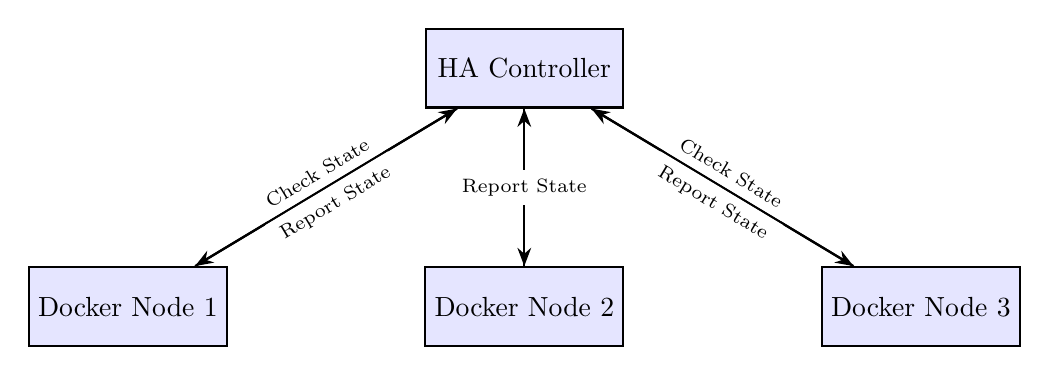
\begin{tikzpicture}[
    node distance=2cm and 2.5cm,
    mynode/.style={draw, thick, fill=blue!10, minimum width=2.5cm, minimum height=1cm, align=center},
    myarrow/.style={-Stealth, thick},
    mylabel/.style={midway, fill=white, font=\scriptsize}
]

  % Nodes
  \node[mynode] (controller) {HA Controller};
  \node[mynode, below left=of controller] (docker1) {Docker Node 1};
  \node[mynode, below=of controller] (docker2) {Docker Node 2};
  \node[mynode, below right=of controller] (docker3) {Docker Node 3};

  % Arrows
  \draw[myarrow] (controller) -- (docker1) node[mylabel, above, sloped] {Check State};
  \draw[myarrow] (controller) -- (docker2) node[mylabel] {Check State};
  \draw[myarrow] (controller) -- (docker3) node[mylabel, above, sloped] {Check State};

  \draw[myarrow] (docker1) -- (controller) node[mylabel, below, sloped] {Report State};
  \draw[myarrow] (docker2) -- (controller) node[mylabel] {Report State};
  \draw[myarrow] (docker3) -- (controller) node[mylabel, below, sloped] {Report State};

\end{tikzpicture}
\caption{High-level architecture of the quantum-inspired HA system.}
\label{fig:system_architecture}
\end{figure}

The diagram represents the high-level architecture of the quantum-inspired High Availability (HA) system.

    \begin{itemize}
        \item HA Controller:
    
        The central node labeled "HA Controller" is the main control unit of the system.
        It manages the HA logic and decision-making process based on the states reported by the Docker nodes.

    \item Docker Nodes:
        The three nodes surrounding the HA Controller represent Docker containers acting as individual nodes in the HA system.
        Each Docker node hosts a simple Python script that simulates a component of the HA system.
        These scripts expose endpoints through which they report their current state (e.g., health and load) to the HA Controller.

    \item Arrows:
        The arrows between the HA Controller and the Docker nodes indicate the flow of information.
        From the HA Controller to the Docker nodes: The controller checks the state of each Docker node by querying their endpoints.
        From the Docker nodes to the HA Controller: The Docker nodes report their states back to the controller after being queried.

   \item  Communication:
        The bidirectional arrows symbolize the communication between the HA Controller and the Docker nodes.
        This communication loop allows the HA Controller to continuously monitor the states of the Docker nodes and make decisions based on their reported states.
\end{itemize}
Each Docker container runs a simple Python script utilizing FastAPI to return the load and health state of the HA system via an endpoint. The HA Controller assigns a probability to each node based on the reported state, implementing HA logic inspired by quantum superposition. This setup contrasts with the daisy chain method, allowing for a one-time parallel processing inspired by the Deutsch-Jozsa algorithm, significantly enhancing decision-making efficiency.

% ------------------------------------------

The objective of this Proof of Concept (POC) is to demonstrate the efficacy of a quantum superposition-inspired model in enhancing High-Availability (HA) systems and load balancing mechanisms. We aim to simulate this model using Docker containers that represent individual nodes within an HA cluster. Each container runs a simple Python script utilizing FastAPI to serve as a microservice, returning data on load and system health. This setup will allow us to assign probabilities to each node, simulating a quantum-inspired selection process. Additionally, we set up a traditional daisy chain method as a control for comparison.

\subsection{Simulation of Nodes using Docker Containers}
The first step in our POC involves creating Docker containers to simulate the nodes within our HA system. Each container will run a Python script with FastAPI, which exposes an endpoint to report simulated load and system health metrics.

\textbf{Step 1: Docker Container Setup}
\begin{enumerate}
    \item Install Docker on a host machine.
    \item Create a Dockerfile that specifies the Python environment, installs FastAPI, and sets up the script to run on container startup.
    \item Build the Docker image using the Dockerfile.
    \item Run multiple instances (containers) from the built image to simulate nodes in the HA system.
\end{enumerate}

\textbf{Step 2: Python Script with FastAPI}
The Python script within each container will:
\begin{enumerate}
    \item Utilize FastAPI to create a simple web server.
    \item Expose an endpoint (e.g., \texttt{/health}) that returns JSON data representing the node's current simulated load and health status.
    \item Incorporate randomness or predefined conditions to simulate variations in load and health.
\end{enumerate}

\subsection{Setup of Logic Controllers Based on Quantum Superposition}
The core of our quantum-inspired model lies in the logic controllers that assess and select nodes based on their reported health and load, akin to the measurement process causing wave function collapse in quantum mechanics.

\textbf{Step 3: Controller Implementation}
\begin{enumerate}
    \item Develop a logic controller that fetches health and load data from each node's FastAPI endpoint.
    \item Implement an algorithm inspired by the Deutsch-Jozsa algorithm, allowing the controller to process nodes' data in parallel, assigning a probability to each node reflecting its suitability for handling incoming requests.
    \item The controller makes a 'measurement' (decision) by selecting a node based on the assigned probabilities, effectively collapsing the superposition of possible node selections to a single choice.
\end{enumerate}

\subsection{Comparison with Daisy Chain Method}
To evaluate the effectiveness of our quantum-inspired approach, we set up a traditional daisy chain method as a control.

\textbf{Daisy Chain Setup}
\begin{enumerate}
    \item Configure the nodes in a sequential order where each node is aware of the next node in the chain.
    \item On failure or high load, the current node passes requests to the next node in the sequence.
\end{enumerate}

\textbf{Comparison and Contrast}
The primary comparison will focus on:
\begin{enumerate}
    \item The time and efficiency in selecting optimal nodes for handling requests.
    \item The system's ability to adapt to changing loads and node health dynamically.
    \item Fault tolerance and system recovery times under various simulated conditions.
\end{enumerate}

\newpage
\section{Examples}
\subsection{HA Controller Example Code}

The HA Controller is the central component of our quantum-inspired HA system. It periodically queries each Docker node for its health and load status and then determines the most suitable node for handling incoming requests. This process is inspired by the quantum superposition principle, where the HA Controller evaluates all possible node states simultaneously and selects the optimal node based on a probabilistic model.

Below is a simplified Python code snippet for the HA Controller. This example utilizes the \texttt{requests} library to send HTTP GET requests to each node's FastAPI endpoint, which returns the node's current load and health status. The controller then uses these reports to assign a probability to each node being the best choice for handling the next request. This decision-making process is analogous to the wave function collapse in quantum mechanics, where the superposition state of nodes collapses to a single state — the selected node.

\begin{lstlisting}[language=Python, caption=HA Controller Python Example]
import requests

# List of Docker node endpoints
node_endpoints = [
    "http://node1.example.com/health",
    "http://node2.example.com/health",
    "http://node3.example.com/health"
]

def get_node_states():
    node_states = {}
    for endpoint in node_endpoints:
        try:
            response = requests.get(endpoint)
            if response.status_code == 200:
                node_states[endpoint] = response.json()['health']
        except requests.RequestException as e:
            print(f"Error fetching state for {endpoint}: {e}")
    return node_states

def select_optimal_node(node_states):
    # Simplified selection logic based on node health
    optimal_node = max(node_states, key=node_states.get)
    return optimal_node

def main():
    node_states = get_node_states()
    optimal_node = select_optimal_node(node_states)
    print(f"Optimal node for handling the next request: {optimal_node}")

if __name__ == "__main__":
    main()
\end{lstlisting}

This example assumes each Docker node's FastAPI application exposes a \texttt{/health} endpoint, returning a JSON object with a 'health' key indicating the node's health status. The HA Controller fetches these states and selects the node with the highest health score as the most suitable for handling incoming requests. The actual implementation may involve more sophisticated selection criteria and error handling to suit specific system requirements.
\subsection{Docker Container Node Examples}
\subsubsection{Example 1: Memory Utilization}

In telephony systems, high memory utilization could lead to degraded performance or even system crashes. This example simulates a Docker container reporting its current memory utilization.

\begin{lstlisting}[language=Python, caption=Memory Utilization FastAPI Application]
from fastapi import FastAPI
from random import randint

app = FastAPI()

@app.get("/memory")
async def memory_utilization():
    memory_used = randint(50, 90)  # Simulated memory usage percentage
    memory_health = 100 - memory_used  # The lower the memory used, the healthier the system
    
    return {"memory_health": memory_health}
\end{lstlisting}

This Python FastAPI application simulates memory utilization of a node within a telephony system. A \texttt{GET} request to the \texttt{/memory} endpoint returns a simulated "memory health" metric, indicating how much memory is free. A healthier system has more free memory, which is crucial for handling spikes in demand.

\subsubsection{Example 2: CPU Load}

Another critical metric for HA systems is CPU load. Overloaded CPUs can result in slow processing times and dropped calls in telephony systems. This example simulates CPU load reporting.

\begin{lstlisting}[language=Python, caption=CPU Load FastAPI Application]
from fastapi import FastAPI
from random import uniform

app = FastAPI()

@app.get("/cpu")
async def cpu_load():
    cpu_usage = uniform(0.5, 0.9)  # Simulated CPU usage (50% to 90%)
    cpu_health = (1 - cpu_usage) * 100  # Health is inversely proportional to CPU usage
    
    return {"cpu_health": cpu_health}
\end{lstlisting}

This application reports a "cpu\_health" metric based on simulated CPU usage. Lower usage results in higher health scores, essential for maintaining system responsiveness.

\subsubsection{Example 3: Network Latency}

Network latency is a vital factor in telephony systems, affecting call quality and system reliability. This example Docker container simulates network latency measurements.

\begin{lstlisting}[language=Python, caption=Network Latency FastAPI Application]
from fastapi import FastAPI
from random import uniform

app = FastAPI()

@app.get("/latency")
async def network_latency():
    latency = uniform(0.1, 0.5)  # Simulated network latency in seconds
    # Assuming a threshold of 0.3 seconds for acceptable latency
    latency_health = 100 - (latency / 0.5) * 100  # Health based on how close to threshold
    
    return {"latency_health": latency_health}
\end{lstlisting}

The "latency\_health" score reflects the proximity of the current latency to acceptable thresholds. Lower latency is ideal, indicating a more responsive system.

These Docker container examples, each running a FastAPI application, simulate various system health metrics for a high-availability telephony system. By querying these endpoints, an HA Controller can make informed decisions on routing or load balancing, enhancing overall system performance and reliability.


\subsection{HA in Active/Active Appliance Cluster Example}

In an active/active appliance cluster, all nodes are active and share the responsibility of handling requests to ensure high availability and load balancing. This scenario requires a dynamic HA/Load Balance Logic Controller to assess the health and load of each node to distribute requests optimally.

\subsubsection{HA/Load Balance Logic Controller}

The Logic Controller plays a crucial role in continuously monitoring the health and load of each node and deciding where to route new incoming requests. Here's a simplified example code for such a controller:

\begin{lstlisting}[language=Python, caption=HA/Load Balance Logic Controller]
import requests

# List of active nodes in the cluster
node_endpoints = [
    "http://node1.example.com/status",
    "http://node2.example.com/status",
    # Add more nodes as needed
]

def fetch_node_status():
    node_status = {}
    for endpoint in node_endpoints:
        try:
            response = requests.get(endpoint, timeout=5)
            if response.status_code == 200:
                node_status[endpoint] = response.json()
            else:
                node_status[endpoint] = {"health": 0, "load": 100}  # Assume max load and no health
        except requests.RequestException:
            node_status[endpoint] = {"health": 0, "load": 100}  # Assume max load and no health
    return node_status

def select_node_for_request(node_status):
    # Example logic: Select the node with the highest health and lowest load
    best_node = min(node_status, key=lambda k: (node_status[k]['load'], -node_status[k]['health']))
    return best_node

def main():
    status = fetch_node_status()
    selected_node = select_node_for_request(status)
    print(f"Selected Node for Incoming Request: {selected_node}")

if __name__ == "__main__":
    main()
\end{lstlisting}

This controller fetches the health and load status from each node and selects the node with the highest health and lowest load to handle incoming requests. It simulates a simple active/active load balancing strategy.

\subsubsection{Docker Node Container Simulation}

Each node in the active/active cluster needs to report its current health and load. The following is an example Python script using FastAPI for a Docker container simulating such a node:

\begin{lstlisting}[language=Python, caption=Docker Node Container Simulation]
from fastapi import FastAPI
from random import randint, random

app = FastAPI()

@app.get("/status")
async def status():
    # Simulated health and load metrics
    health = random()  # Random health metric, 0 (unhealthy) to 1 (healthy)
    load = randint(0, 100)  # Random load percentage, 0% to 100%
    
    return {"health": health, "load": load}
\end{lstlisting}

Each node simulates its health and load metrics, which the HA/Load Balance Logic Controller uses to make routing decisions. This setup ensures that requests are distributed evenly, maintaining high availability and performance across the cluster.


\subsection{High Availability VoIP Subsystem Example}

This example focuses on a High Availability (HA) VoIP system designed to offer enhanced availability and efficient failure recovery when interfacing with the PSTN or other TDM networks. The architecture of such a system involves multiple gateways and at least one central hub, each equipped with a proxy table and a call restoration table to facilitate robust call handling and recovery.

\subsubsection{System Architecture and Components}

The HA VoIP system architecture includes the following components:

\begin{itemize}
    \item \textbf{Gateways:} Multiple gateways serve as the primary interface between the PSTN and the VoIP system. Each gateway is configured with a proxy table and a call restoration table.
    \item \textbf{Hub:} At least one hub centralizes key VoIP services, including a proxy server for handling SIP (Session Initiation Protocol) portions of calls and a media server for managing RTP (Real-Time Protocol) portions.
    \item \textbf{Proxy Server:} Located within the hub, it handles the SIP portion of calls, facilitating call setup and management.
    \item \textbf{Media Server:} Also within the hub, it processes the RTP portion, responsible for the actual transmission of voice data.
    \item \textbf{SIP Controlled Softphones:} Endpoints that receive routed SIP voice calls, enabling voice communication.
\end{itemize}

\subsubsection{Operational Flow}

The operational flow for handling an incoming call involves several steps:

\begin{enumerate}
    \item An incoming call from the PSTN is received by one of the gateways.
    \item The call is divided into two portions: SIP (for call control) and RTP (for media/voice data).
    \item The SIP portion is forwarded to the proxy server, and the RTP portion is sent to the media server, both located in the hub.
    \item The proxy server and media server process their respective portions and route them to the intended endpoint, such as a SIP-controlled softphone.
    \item In case of gateway failure, the proxy table and call restoration table within each gateway facilitate quick recovery and rerouting of calls to ensure continuous service.
\end{enumerate}

\subsubsection{High Availability and Failure Recovery}

The system ensures high availability and robust failure recovery through:

\begin{itemize}
    \item \textbf{Proxy Table and Call Restoration Table:} These configurations in each gateway enable intelligent call routing and rapid recovery from failures, minimizing service disruption.
    \item \textbf{Multiple Gateways:} The use of multiple gateways offers redundancy, allowing the system to reroute calls through alternate gateways if one fails.
    \item \textbf{Priority Table for Proxy Servers:} This allows the system to prioritize which proxy server to use for routing SIP calls, further enhancing the system's resilience and flexibility.
\end{itemize}

This HA VoIP system exemplifies how sophisticated routing and recovery mechanisms can significantly enhance the reliability and availability of VoIP services, especially in critical communication infrastructures interfacing with traditional telephony networks.

\subsection{High Availability VoIP Subsystem Example}

This example explores the implementation of a high availability Voice over IP (VoIP) system. Our POC simulates a VoIP environment interfacing with traditional telephony networks to enhance availability and improve failure recovery. The setup includes simulating multiple gateways coupled to a central hub, along with proxy and call restoration tables configured within each gateway.

\subsubsection{Simulating VoIP Gateways}

Each simulated VoIP gateway is represented by a Docker container running a FastAPI application. These gateways interface with the simulated Public Switched Telephone Network (PSTN) and process VoIP calls, separating them into Session Initiation Protocol (SIP) and Real-Time Protocol (RTP) portions.

\begin{lstlisting}[language=Python, caption=Simulated VoIP Gateway FastAPI Application]
from fastapi import FastAPI
from typing import Dict

app = FastAPI()

@app.post("/call")
async def process_call(call_data: Dict):
    # Simulate dividing a call into SIP and RTP portions
    sip_portion = {"type": "SIP", "data": call_data["sip_data"]}
    rtp_portion = {"type": "RTP", "data": call_data["rtp_data"]}
    
    # Simulated sending to proxy server and media server
    proxy_server_response = send_to_proxy_server(sip_portion)
    media_server_response = send_to_media_server(rtp_portion)
    
    return {"proxy_server": proxy_server_response, "media_server": media_server_response}

def send_to_proxy_server(sip_data):
    # Placeholder for sending SIP data to a simulated proxy server
    return {"status": "success", "message": "SIP data processed"}

def send_to_media_server(rtp_data):
    # Placeholder for sending RTP data to a simulated media server
    return {"status": "success", "message": "RTP data processed"}
\end{lstlisting}

\subsubsection{Configuring Proxy and Call Restoration Tables}

In our simulated environment, each gateway contains a proxy table and a call restoration table, essential for managing call routing and recovery.

\begin{lstlisting}[language=Python, caption=Configuration of Proxy and Call Restoration Tables]
# Example Python code snippet for configuring proxy and call restoration tables in a gateway

proxy_table = {
    "gateway1": {"priority": 1, "proxy_server": "ProxyServer1"},
    "gateway2": {"priority": 2, "proxy_server": "ProxyServer2"},
    # Additional gateways as needed
}

call_restoration_table = {
    "call_id_1": {"original_gateway": "gateway1", "backup_gateway": "gateway2"},
    "call_id_2": {"original_gateway": "gateway2", "backup_gateway": "gateway1"},
    # Additional call mappings as needed
}
\end{lstlisting}

\subsubsection{Routing Calls Through the VoIP System}

The system uses the proxy server priority table to route SIP voice calls through the VoIP gateways efficiently. This routing ensures high availability by dynamically selecting the optimal path for each call based on current gateway states and proxy server priorities.

```latex
This setup outlines how a high availability VoIP subsystem could be simulated using Docker containers for gateways, each running a FastAPI application to mimic the functionalities of real-world VoIP gateways. The configurations and routing logic presented aim to enhance understanding of managing VoIP calls in a high-availability environment.

\subsection{High Availability and Disaster Recovery for Computing Systems}

This example outlines a strategy for enhancing high availability and disaster recovery within computing systems, particularly focusing on virtual computing environments. The approach employs Docker containers to simulate different components of a computing system and an HA/Load Balance Logic Controller to manage the system's resilience and response to failures.

\subsubsection{HA/Load Balance Logic Controller}

The HA/Load Balance Logic Controller plays a pivotal role in monitoring the health of the system's components and effectively managing disaster recovery processes. Below is a conceptual Python code snippet illustrating how such a controller might operate:

\begin{lstlisting}[language=Python, caption=HA/Load Balance Logic Controller for Disaster Recovery]
import requests

# Endpoints for simulated components of the computing system
component_endpoints = [
    "http://component1.example.com/status",
    "http://component2.example.com/status",
    # Additional components as needed
]

def check_system_health():
    health_status = {}
    for endpoint in component_endpoints:
        try:
            response = requests.get(endpoint, timeout=3)
            health_status[endpoint] = 'Online' if response.status_code == 200 else 'Offline'
        except requests.RequestException:
            health_status[endpoint] = 'Offline'
    return health_status

def initiate_recovery(offline_components):
    for component in offline_components:
        print(f"Initiating recovery process for {component}...")
        # Simulate a recovery action
        # In a real scenario, this might involve restarting services, switching to backup systems, etc.

def main():
    system_health = check_system_health()
    offline_components = [comp for comp, status in system_health.items() if status == 'Offline']
    
    if offline_components:
        initiate_recovery(offline_components)
    else:
        print("All system components are operational.")

if __name__ == "__main__":
    main()
\end{lstlisting}

This logic controller periodically checks the health status of each system component. If any component is found to be offline, it triggers a recovery process aimed at restoring the component's functionality, ensuring the system's high availability and robustness against disasters.

\subsubsection{Docker Container Simulation for System Components}

To simulate the protected computing system's components, each Docker container runs a lightweight application to mimic the behavior of system parts (e.g., servers, storage units) in a virtual computing environment. The example below represents a simple simulation:

\begin{lstlisting}[language=Python, caption=Docker Container Simulation for System Components]
from fastapi import FastAPI
import uvicorn

app = FastAPI()

@app.get("/status")
def status():
    # Simulate component health check
    # In a real scenario, this might involve checking service status, resource usage, etc.
    return {"status": "Online"}

if __name__ == "__main__":
    uvicorn.run(app, host="0.0.0.0", port=8000)
\end{lstlisting}

Each containerized component exposes a `/status` endpoint, allowing the HA/Load Balance Logic Controller to ascertain the component's operational status. This setup forms the basis for a resilient computing system capable of high availability and efficient disaster recovery.


\subsection{Quantum Superposition-Based HA in Multi-Node Storage Cluster}

Leveraging quantum superposition principles, this POC introduces a novel approach to ensuring high availability in a multi-node storage cluster. The system dynamically manages NVRAM mirroring and HA partner relationships utilizing a Quantum Superposition HA Controller (QSHAC). This controller evaluates and rebalances the cluster's state in response to changes, optimizing data resilience and access speed.

\subsubsection{Quantum Superposition HA Controller (QSHAC)}

The QSHAC embodies the quantum-inspired decision-making process, evaluating all possible node states and their combinations to optimally redistribute storage loads and manage NVRAM mirroring across the cluster.

\begin{lstlisting}[language=Python, caption=Quantum Superposition HA Controller]
import requests
from quantum_logic import QuantumDecisionProcess  # Hypothetical module

node_endpoints = [
    "http://node1.example.com/nvram",
    "http://node2.example.com/nvram",
    # Additional nodes as needed
]

def fetch_nvram_states():
    states = {}
    for endpoint in node_endpoints:
        response = requests.get(f"{endpoint}/state")
        states[endpoint] = response.json()['state']
    return states

def quantum_mirror_decision(states):
    decision_maker = QuantumDecisionProcess(states)
    mirroring_plan = decision_maker.optimal_mirroring_strategy()
    return mirroring_plan

def main():
    states = fetch_nvram_states()
    mirroring_plan = quantum_mirror_decision(states)
    for source, target in mirroring_plan.items():
        mirror_nvram(source, target)

if __name__ == "__main__":
    main()
\end{lstlisting}

The controller uses a hypothetical `QuantumDecisionProcess` module to calculate the optimal NVRAM mirroring strategy, akin to evaluating quantum states in superposition and determining the best state through wave function collapse.

\subsubsection{Docker Node Container with Simulated NVRAM}

Each Docker container simulates a storage node with NVRAM. It supports operations to read and write NVRAM state, simulating the data mirroring process influenced by the QSHAC's decisions.

\begin{lstlisting}[language=Python, caption=Docker Node Container with Simulated NVRAM]
from fastapi import FastAPI

app = FastAPI()

nvram = {"state": "initial"}

@app.get("/nvram")
def read_nvram():
    return nvram

@app.post("/nvram")
def write_nvram(data: dict):
    global nvram
    nvram = data
    return {"message": "NVRAM state updated"}

@app.get("/state")
def get_state():
    # Simulate determining the node's state for the QSHAC
    return {"state": nvram['state']}
\end{lstlisting}

In this POC, the Docker nodes and the QSHAC work in concert to dynamically manage the cluster's HA configuration. By simulating quantum superposition and decision-making processes, the system ensures that NVRAM data is mirrored across the cluster in the most resilient and efficient manner, akin to achieving high availability through quantum computing principles.

\section{Integrating MBX with QSHAC}

Integrating a Session Initiation Protocol (SIP) server or a software-based Automatic Call Distributor (ACD), designated as MBX and hosted on a virtual machine, into the Quantum Superposition High Availability Controller (QSHAC) framework involves several critical steps. The QSHAC, inspired by quantum computing concepts, especially quantum superposition, aims to optimize the decision-making process for high availability in telephony systems. This process ensures that incoming communication requests are routed to the most suitable MBX instance based on real-time assessments of system health and load.

\paragraph{Representation of MBX Instances as Quantum States:} Each MBX instance, representing a potential SIP server or soft ACD, is analogous to a quantum state within the QSHAC's decision-making matrix. These instances can be denoted as \(|MBX_1\rangle\), \(|MBX_2\rangle\), ..., \(|MBX_n\rangle\), where each state \(|MBX_i\rangle\) corresponds to a unique configuration or operational condition of the MBX. The superposition of these states, represented as \(|\psi\rangle = \sum_{i} a_i |MBX_i\rangle\), where \(a_i\) are probability amplitudes, reflects the composite operational landscape of the MBX instances.

\paragraph{Health Metrics and Quantum Measurement:} In quantum mechanics, the act of measurement collapses a superposed state into a definite state; similarly, QSHAC evaluates the 'health' of each MBX instance through specific metrics, such as call handling capacity, response times, or error rates. This evaluation process, akin to quantum measurement, collapses the superposed operational landscape \(|\psi\rangle\) into a definitive choice \(|MBX_k\rangle\) for routing new communication requests, based on the computed probabilities derived from health metrics.

\paragraph{Dynamic Configuration for High Availability:} The dynamic nature of QSHAC allows for real-time reconfiguration of MBX instances in response to varying operational demands and system health. This flexibility ensures that the telephony system remains highly available, with SIP traffic and call distribution being optimally managed across the MBX instances. In the event of an MBX instance's degradation or failure, QSHAC can swiftly reroute traffic to other healthier instances, minimizing disruption and maintaining service quality.

\paragraph{Event-Driven System Adaptation:} QSHAC operates on an event-driven basis, continuously monitoring the system for changes in configuration, node addition or removal, and other significant events that may affect system availability. Upon detecting such events, QSHAC recalibrates the health assessments and probability amplitudes \(a_i\) for the MBX instances, ensuring that the system's operational state remains optimally aligned with the current conditions.

Integrating MBX with QSHAC not only enhances the resilience and availability of telephony systems but also introduces a level of operational flexibility and efficiency that traditional high availability solutions may not provide. This quantum-inspired approach allows for sophisticated, probabilistic management of system resources, ensuring that each communication request is handled by the most suitable MBX instance at any given moment.


\subsubsection{Defining MBX's Microservices}

Each microservice within MBX can be represented as a quantum state, or "ket", in the QSHAC's decision-making model. For instance, if we consider two primary microservices of MBX responsible for SIP session initiation (\(|SIP\rangle\)) and real-time protocol handling (\(|RTP\rangle\)), the overall system state (\(|\psi\rangle\)) could be represented as a superposition of these states:

\[|\psi\rangle = a|SIP\rangle + b|RTP\rangle\]

where \(a\) and \(b\) are coefficients that represent the probability amplitudes of each microservice being in an optimal operational state. The values of \(a\) and \(b\) are determined by the microservices' health and load metrics.

\subsubsection{Virtualization Benefits}

MBX's virtual environment facilitates dynamic allocation of computational resources. Virtualization allows MBX to adapt its resource allocation in real-time, enhancing its throughput and response to demand fluctuations—crucial for maintaining service quality.

\subsubsection{Interfacing MBX with QSHAC}

To effectively integrate MBX with QSHAC, an API is developed, enabling QSHAC to query MBX's microservices' states and to make routing decisions based on the quantum superposition model. This interface acts as the measurement process in quantum mechanics, collapsing the system's superposition state into a particular configuration based on the QSHAC's analysis.

\subsubsection{Quantum Superposition Model Implementation}

QSHAC represents the various operational configurations of MBX's microservices as quantum states in superposition. For instance, during high demand periods, the system state may shift towards \(|RTP\rangle\) to ensure optimal call quality:

\[|\psi_{high\ demand}\rangle = a'|SIP\rangle + b'|RTP\rangle\]

where \(b' > a'\), reflecting a greater emphasis on RTP handling.

\subsubsection{Dynamic Resource Allocation}

Based on QSHAC's decisions, MBX dynamically adjusts its resources, ensuring that microservices are configured optimally. This dynamic adjustment is akin to the quantum measurement outcome affecting the system's state in quantum mechanics.

\subsubsection{Continuous Monitoring and Adjustment}

QSHAC's continuous monitoring system is akin to repeatedly measuring a quantum system's state, ensuring MBX's operational configuration remains optimal. Adjustments are made in real-time, akin to wave function collapse, based on the latest system state assessments.

\subsubsection{Requirements for Integration}

\begin{itemize}
    \item Understanding of quantum states and superposition.
    \item Skills in API development for QSHAC-MBX communication.
    \item Expertise in managing and optimizing virtual machines.
    \item Capability to implement continuous monitoring and dynamic resource allocation mechanisms.
\end{itemize}

This integration not only capitalizes on MBX's virtualized, microservices-based architecture but also introduces a novel approach to high availability management using quantum-inspired models, enhancing SIP servers and soft ACD systems' reliability and efficiency.

\subsubsection{Flowchart Representation}

\begin{figure}[ht]
\centering
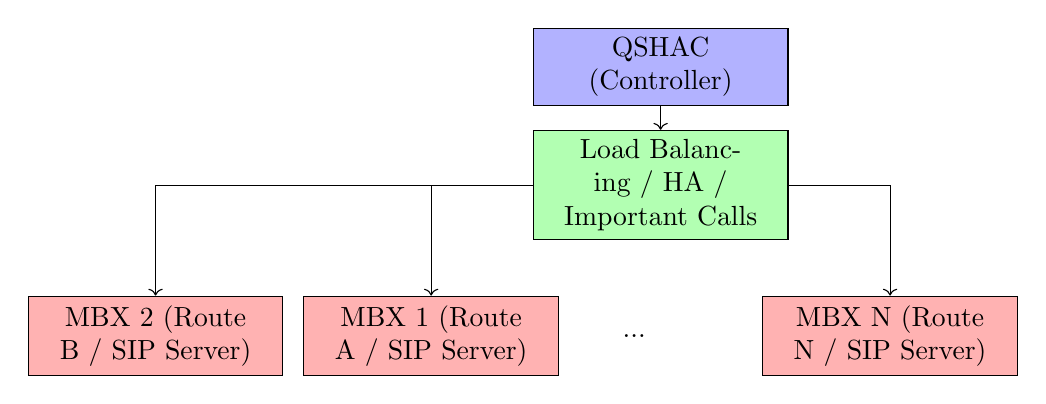
\begin{tikzpicture}[node distance=2cm]
    \node (qshac) [rectangle, draw, text width=3cm, text centered, fill=blue!30] {QSHAC (Controller)};
    \node (lbha) [below of=qshac, rectangle, draw, text width=3cm, text centered, fill=green!30, yshift=0.5cm] {Load Balancing / HA / Important Calls};
    \node (mbx1) [below left of=lbha, rectangle, draw, text width=3cm, text centered, fill=red!30, xshift=-1.5cm, yshift=-0.5cm] {MBX 1 (Route A / SIP Server)};
    \node (mbx2) [left of=mbx1, rectangle, draw, text width=3cm, text centered, fill=red!30, xshift=-1.5cm] {MBX 2 (Route B / SIP Server)};
    \node (mbxn) [below right of=lbha, rectangle, draw, text width=3cm, text centered, fill=red!30, xshift=1.5cm, yshift=-0.5cm] {MBX N (Route N / SIP Server)};
    \node (dots) [left of=mbxn, xshift=-1.25cm] {...};

    \draw [->] (qshac) -- (lbha);
    \draw [->] (lbha) -| (mbx1);
    \draw [->] (lbha) -| (mbx2);
    \draw [->] (lbha) -| (mbxn);
\end{tikzpicture}
\caption{Flowchart depicting the integration of MBX with QSHAC.}
\end{figure}

In this architecture, the QSHAC operates as the central decision-maker, assessing the state of each MBX instance for optimal call routing based on high availability, load conditions, and call priority. Each MBX instance, equipped with microservices including the SIP server, is prepared to handle SIP sessions and RTP media processing efficiently. The system's design facilitates dynamic scalability and resource allocation, ensuring high-quality service delivery and system resilience.

The integration showcases how virtualization and microservices architecture, combined with quantum-inspired decision-making, can revolutionize telephony systems' efficiency and reliability.


\end{document}






\section{System Overview}
\subsection{High-Level Architecture}
Describe the architecture of the HA system, highlighting the role of Docker containers simulating nodes and a central controller determining node health and selecting the active node.

% Placeholder for System Architecture Diagram
\begin{figure}[h]
    \centering
    \includegraphics[width=0.8\textwidth]{system_architecture.png}
    \caption{High-level architecture of the quantum-inspired HA system.}
    \label{fig:system_architecture}
\end{figure}

\subsection{Components}
\subsubsection{Docker Containers as Nodes}
Explain how Docker containers are utilized to simulate individual nodes within the HA system, each running a FastAPI application to expose health metrics.

\subsubsection{FastAPI Application for Node Health Simulation}
Detail the FastAPI application's role within Docker containers, particularly its function in simulating node health and exposing this data through an API endpoint.

\begin{lstlisting}[language=Python, caption=FastAPI Application for Node Health Simulation]
from fastapi import FastAPI
from random import random

app = FastAPI()

@app.get("/health")
async def health():
    # Simulate node health metric
    health_score = random()
    return {"health_score": health_score}
\end{lstlisting}

\subsubsection{HA Controller}
Describe the Python script acting as the HA controller, periodically polling node health from the FastAPI endpoints and selecting the active node based on computed probabilities.

\section{Implementation}
\subsection{Setting Up Docker Containers}
Guide on setting up Docker containers, each running a FastAPI app for node simulation.

\subsection{Simulating Node Health with FastAPI}
Instructions and code for creating the FastAPI application to simulate and expose node health metrics.

\subsection{HA Decision Mechanism}
Describe the implementation of the HA controller's decision algorithm, using Python to select the active node based on health scores.

\section{Diagrams}
Provide detailed text descriptions of the internal mechanisms of each block and include placeholders for flow diagrams illustrating these processes.

% Placeholder for Flow Diagram of Node Health Simulation
\begin{figure}[h]
    \centering
    \includegraphics[width=0.8\textwidth]{node_health_simulation_flow.png}
    \caption{Flow diagram illustrating the node health simulation process.}
    \label{fig:node_health_simulation_flow}
\end{figure}

\section{Conclusion}
Summarize the POC's objectives, achieved outcomes, and potential areas for future exploration.

\end{document}
